\documentclass[t]{beamer}
%\documentclass{beamer}
\listfiles

\mode<presentation>
{
  \usetheme[deutsch,titlepage0]{KIT}
% \usetheme[usefoot]{KIT}
% \usetheme{KIT}

%%  \usefonttheme{structurebold}

  \setbeamercovered{transparent}

  %\setbeamertemplate{enumerate items}[circle]
  \setbeamertemplate{enumerate items}[ball]

}
\usepackage{babel}
%\date{10.05.2010}
%\DateText

\newlength{\Ku}
\setlength{\Ku}{1.43375pt}

\usepackage[utf8]{inputenc}
\usepackage[TS1,T1]{fontenc}
\usepackage{array}
\usepackage{multicol}
\usepackage{lipsum}
\usepackage{xspace}
\usepackage{listings}
\usepackage[sort&compress]{natbib}
\usepackage{inconsolata}
\usepackage[scaled]{beramono}

%\usenavigationsymbols
%\usenavigationsymbols[sfHhdb]
%\usenavigationsymbols[sfhHb]

\title[]{Integration von Transactional Memory in Hochsprachen}
\subtitle{
Niklas Baumstark\\
Proseminar „Transactional Memory“}

\author[]{Niklas Baumstark}

\AuthorTitleSep{}

\institute[]{Lehrstuhl für Rechnerarchitektur und Parallelverarbeitung, Prof. Karl}

\TitleImage[width=\titleimagewd]{Bilder/KIT-Titel}

\newlength{\tmplen}

\newcommand{\verysmall}{\fontsize{6pt}{8.6pt}\selectfont}

\newcommand{\Rplus}{\protect\raisebox{.1ex}{+}}
\newcommand{\Cpp}{\mbox{C\Rplus\Rplus}\xspace}
\newcommand{\CppEleven}{\mbox{C\Rplus\Rplus11}\xspace}
\newcommand{\CppNext}{\mbox{C\Rplus\Rplus1x}\xspace}

\lstset{basicstyle=\footnotesize\ttfamily,
        numbers=none,
        numberstyle=\scriptsize,
        numbersep=5pt,
        tabsize=4,
        captionpos=b,
        framexleftmargin=1mm,
        escapeinside={\%*}{*)},
  }
\lstset{literate=%
  {Ö}{{\"O}}1
  {Ä}{{\"A}}1
  {Ü}{{\"U}}1
  {ß}{{\ss}}2
  {ü}{{\"u}}1
  {ä}{{\"a}}1
  {ö}{{\"o}}1
}

\bibliographystyle{plain}
\KITfoot{\parbox[t]{150mm}{
  \vspace{0.1em} \tiny
  \today
  \qquad\qquad\qquad\qquad\qquad\qquad\qquad\qquad \textbf{Niklas Baumstark - Integration von TM in Hochsprachen}
  \qquad\qquad\qquad\qquad\qquad\qquad\qquad\qquad ITEC
}}

%\setbeamertemplate{footline}
%{
  %\leavevmode%
  %\hbox{%
  %\begin{beamercolorbox}[wd=.333333\paperwidth,ht=2.25ex,dp=1ex,center]{author in head/foot}%
    %\usebeamerfont{author in head/foot}\insertshortauthor%~~\beamer@ifempty{\insertshortinstitute}{}{(\insertshortinstitute)}
  %\end{beamercolorbox}%
  %\begin{beamercolorbox}[wd=.333333\paperwidth,ht=2.25ex,dp=1ex,center]{title in head/foot}%
    %\usebeamerfont{title in head/foot}\insertshorttitle
  %\end{beamercolorbox}%
  %\begin{beamercolorbox}[wd=.333333\paperwidth,ht=2.25ex,dp=1ex,right]{date in head/foot}%
    %\usebeamerfont{date in head/foot}\insertshortdate{}\hspace*{2em}
    %\insertframenumber{} / \inserttotalframenumber\hspace*{2ex}
  %\end{beamercolorbox}}%
  %\vskip0pt%
%}

\begin{document}

\begin{frame}
  \maketitle
\end{frame}

\begin{frame}
  \frametitle{Gliederung}
  \begin{itemize}
    \item Motivation
    \item \Cpp
      \begin{itemize}
      \item Designziele, Standardisierung
      \item Semantik
      \item Syntax
      \item Optimierungen
      \end{itemize}
    \item Haskell
      \begin{itemize}
      \item Kurzer "Uberblick
      \item Beispiel
      \end{itemize}
  \end{itemize}
\end{frame}

\section{Motivation}
\begin{frame}[fragile]
  \frametitle{Motivation}

  \begin{itemize}
  \item TM deutlich einfachere Abstraktion als Locks:
    \begin{itemize}
    \item \lstinline|atomic { ... }| und fertig! (zumindest in der Theorie)
    \end{itemize}
  \item Aber wie dem Programmierer zur Verf"ugung stellen?
    \begin{itemize}
    \item Implementierung: Bibliothek vs. Compiler-/Runtimeintegration
    \item Syntax: optional Spracherweiterung/Pragmas
    \item Einfachkeit vs. viel Kontrolle (Performance!)
    \end{itemize}
  \item Beispiele: \Cpp, Haskell
  \end{itemize}

\end{frame}

\section{Konkrete Beispiele}
\subsection{\Cpp}

%\begin{frame}[fragile]
  %\frametitle{TM in \Cpp (Starke Atomizit"at vs. SLA)}
  %\begin{center}
  %\begin{tabular}{| c || c |} \hline
  %Thread 1 & Thread 2 \\ \hline

%\begin{lstlisting}
%int main() {
%}
%\end{lstlisting}

  %&

%\begin{lstlisting}
%int main() {
%}
%\end{lstlisting}

  %\\
  %\hline
  %\end{tabular}
  %\end{center}
%\end{frame}

\begin{frame}
  \frametitle{TM in \Cpp}

  \begin{itemize}
  \item Designziele:
    \begin{itemize}
    \item Geschwindigkeit
    \item Flexibilit"at (\Cpp wird auf vielen Plattformen eingesetzt)
    \item beliebige Speicherzugriffe in Transaktionen
    \item \Cpp-Sprachelemente unterst"utzen (Templates, Funktionszeiger, Methoden)
    \end{itemize}
  \item SG5 besch"aftigt sich mit der Integration von TM in \CppNext \cite{SG5Status}
  \item Basis: Spezifikations-Draft \cite{C++TMDraft-1.1}
        (u.a. unterst"utzt von GCC 4.7 und Intel STM Compiler)
  \item Grundlegendes Design
    \begin{itemize}
    \item Direkte Spracherweiterung f"ur nahtlose Integration (keine Pragmas)
    \item Compiler instrumentiert transaktionalen Code \\
          $\Rightarrow$ Load-/Store-Funktionsaufrufe an eine TM-Runtime
    \item ABI der Runtime in \cite{TMABI-1.1} genau spezifiziert
    \end{itemize}
  \end{itemize}

\end{frame}

\lstset{language=C++}
\begin{frame}[fragile]
  \frametitle{TM in \Cpp (Semantik)}

  \begin{itemize}
  \item Problematisch: Starke Atomarit"at
    \begin{itemize}
    \item keine Zwischenergebnisse einer Transaktion sind f"ur andere Threads sichtbar \\
          $\Rightarrow$ Also komplettes Programm instrumentieren?
    \end{itemize}
  \item Einfacher: Single-Lock Atomicity (SLA) \cite{TMSemanticsC++}
    \begin{itemize}
    \item Programm verh"alt sich so, als ob ein globales Lock zur Serialisierung
          aller Transaktionen verwendet w"urde
    \item I/O und Legacy-Code ist erlaubt
    \item Probleme: Zur"uckrollen unm"oglich, Isolationseigenschaft nicht garantiert
    \end{itemize}
  \end{itemize}

  \begin{center}
  \begin{tabular}{| l || l |} \hline
  \multicolumn{2}{|c|}{Geteilt: \lstinline|atomic<int> x(0);|} \\ \hline
  Thread 1 & Thread 2 \\ \hline

  \vtop{\null\hbox{\begin{lstlisting}
transaction {
  x = 1;


  while (x == 1) { }
}
  \end{lstlisting}}}

  &

  \vtop{\null\hbox{\begin{lstlisting}


while (x == 0) { }
x = 0;
  \end{lstlisting}}}

  \\
  \hline
  \end{tabular}
  \end{center}

\end{frame}

\begin{frame}[fragile]
  \frametitle{TM in \Cpp (Syntax)}

  \begin{itemize}
  \item \lstinline|__transaction_relaxed { ... }| mit SLA-Semantik
    \begin{itemize}
    \item Kann beliebige Anweisungen enthalten
    \item evtl. Wechsel in einen seriellen Ausf"uhrungsmodus
          (Funktionsaufruf an die Runtime)
    \end{itemize}
  \item \lstinline|__transaction_atomic { ... }| mit st"arkerer Semantik
    \begin{itemize}
    \item atomar im Kontext des Gesamtprogramms
    \item k"onnen mit \lstinline|__transaction_cancel| abgebrochen werden
    \item keine irreversible Operationen (I/O, Aufrufe nicht instrumentierter
          Funktionen, Synchronisationsprimitiven)
    \end{itemize}
  \item Transaktionen k"onnen geschachtelt werden (Ausnahme:
         \lstinline|relaxed| nicht innerhalb von \lstinline|atomic|)
  \item Ausdr"ucke und Funktionen k"onnen Transaktionen sein!
  \end{itemize}

  \begin{center}
  \begin{lstlisting}
int x = 1;
int y = __transaction_atomic (x + 1);
  \end{lstlisting}
  \end{center}
\end{frame}

\begin{frame}[fragile]
  \frametitle{TM in \Cpp (Codebeispiel)}

  \vspace{-1em}
  \begin{lstlisting}
  void inc(int& x) { ++x; }
  void plustwo(int& x) { inc(x); inc(x); }

  int main() {
      int x = 0, y = 0;
      __transaction_atomic {
          plustwo(x);
          y = x; // x = y = 2
          __transaction_atomic {
              y += 2;
              if (y > 3)
                  __transaction_cancel;
          }
      }
      __transaction_relaxed {
          std::cout << y << "\n";
      }
  }
  \end{lstlisting}

  \begin{lstlisting}
  $ g++ -std=c++11 -fgnu-tm test.cpp && ./a.out
  2
  \end{lstlisting}
\end{frame}

\begin{frame}[fragile]
  \frametitle{TM in \Cpp (Ung"ultige Codebeispiele)}

  \begin{lstlisting}
  int main() {
      atomic<int> i(0);
      __transaction_atomic {
          i = 1;
      }
  }
  \end{lstlisting}

  \begin{lstlisting}
  $ g++ -std=c++11 -fgnu-tm test.cpp
  test.cpp:2:14: error: unsafe function call
  'std::__atomic_base<...>::operator=(...)' within atomic transaction
  \end{lstlisting}

  \begin{center}
  \begin{tabular}{| l || l |} \hline
  \multicolumn{2}{|c|}{Geteilt: \lstinline|int x = 0;|} \\ \hline
  Thread 1 & Thread 2 \\ \hline

  \vtop{\null\hbox{\begin{lstlisting}
__transaction_atomic {
    x = 1;
}
  \end{lstlisting}}}

  &

  \vtop{\null\hbox{\begin{lstlisting}

x = 2;

  \end{lstlisting}}}

  \\
  \hline
  \end{tabular}
  \end{center}
\end{frame}

\begin{frame}[fragile]
  \frametitle{TM in \Cpp (Optimierungen)}

  \begin{itemize}
  \item Compiler wei"s durch statische Analyse viel "uber den Datenfluss. \\
        Naive Load-/Store-Funktionsaufrufe an TM-Runtime verhindern aber Optimierung
  \item Idee \cite{DesignAndImplTMC++}: Nicht nur generische
        \lstinline|read|/\lstinline|write|-Operationen,
        sondern auch \lstinline|read_after_read|, \lstinline|write_after_write|,
        \lstinline|read_after_write|, \lstinline|read_for_write|
  \item Compiler teilt so sein Wissen der Runtime mit
  \end{itemize}

  \begin{center}
  \begin{tabular}{| c | c | c | c | c |} \hline
  Code & Repr"asentation & Schritt 1 & Schritt 2 & Schritt 3 \\ \hline

\begin{lstlisting}
y = x
x = x + y
return x
\end{lstlisting}

  &

\begin{lstlisting}
read(x)
write(y)
read(x)
read(y)
write(x)
read(x)
\end{lstlisting}

  &

\begin{lstlisting}
read(x)
write(y)
readAR(x)
readAW(y)
writeAR(x)
readAW(x)
\end{lstlisting}

  &

\begin{lstlisting}
read(x)
write(y)
writeAR(x)
\end{lstlisting}

  &

\begin{lstlisting}
readFW(x)
write(y)
writeAW(x)
\end{lstlisting}

  \\
  \hline
  \end{tabular}
  \end{center}
\end{frame}

\lstset{language=Haskell}

\begin{frame}
  \frametitle{TM in der funktionalen Programmierung}
  \begin{itemize}
    \item FP hat Vorteile in Bezug auf Parallelisierung und STM
          (z.B. Persistente Datenstrukturen)
    \item Aber: Programme kommen nicht komplett ohne ver"anderlichen Zustand aus
    \item Clojure, Haskell bieten erprobte STM-Bibliotheken
    \item Haskell
      \begin{itemize}
      \item pur funktionale Programmiersprache, Seiteneffekte durch spezielle
            Typen (Monaden) repr"asentiert
      \item GHC (Glasgow Haskell Compiler): Green Threads und nichtblockierendes I/O
            $\Rightarrow$ eine Million Threads kein Problem
      \item seit 2006: STM-Bibliothek in Kooperation mit der GHC-Runtime
      \end{itemize}
  \end{itemize}
\end{frame}

\begin{frame}[fragile]
  \frametitle{Haskell's STM}

  \begin{itemize}
  \item Wert vom Typ \lstinline|STM a| ist eine Transaktion, die einen Wert vom Typ
        \lstinline|a| produziert
  \item Transaktionen arbeiten auf Variablen vom Typ \lstinline|TVar a|
  \item \lstinline|retry| bricht Transaktion ab und f"uhrt sie erneut aus
  \item Klassisches Beispiel: Banktransaktion
    \begin{lstlisting}
    transfer :: TVar Int -> TVar Int -> Int -> STM ()
    transfer from to amount = do x1 <- readTVar from
                                 x2 <- readTVar to
                                 when (x1 < amount) retry
                                 writeTVar from (x1 - amount)
                                 writeTVar to (x2 + amount)
    \end{lstlisting}
  \item Seiteneffektfreiheit der Transaktionen wird durch Typsystem forciert:
        I/O-Aktionen sind vom Typ \lstinline|IO a|, es existiert keine Funktion
           \lstinline|IO a -> STM a|
  \item Der umgekehrte Weg existiert: \lstinline|atomically :: STM a -> IO a|
  \end{itemize}
\end{frame}

\begin{frame}[fragile]
  \frametitle{Haskell's STM}

  \begin{itemize}
  \item Neben \lstinline|TVar| z.B. Queues (\lstinline|TChan|) und \lstinline|TMVar|s
        (sind leer oder enthalten ein Datum)
  \item Kombinatoren wie \lstinline|orElse :: STM a -> STM a -> STM a|
  \end{itemize}

  \begin{lstlisting}
    type Event = TMVar ()

    waitFor :: Event -> STM ()
    waitFor evt = takeTMVar evt

    trigger :: Event -> STM ()
    trigger evt = putTMVar evt ()

    buttonClick :: Event
    keyPress :: Event

    waitForUserInput = waitFor buttonClick `orElse` waitFor keyPress
  \end{lstlisting}
\end{frame}

\begin{frame}[fragile]
  \frametitle{Haskell STM vs. Locking}
  \begin{figure}[!t]
    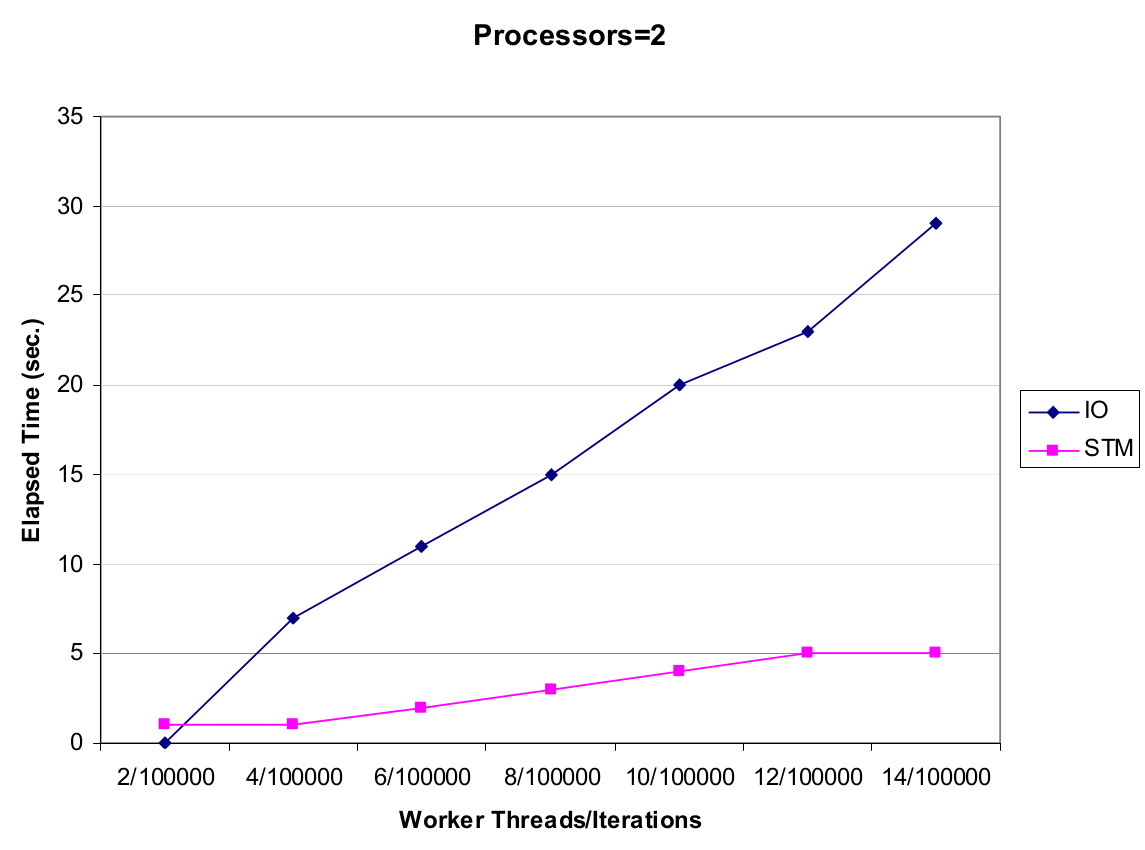
\includegraphics[width=200px]{haskell_stm.png}
    \label{fig:haskell_stm}
  \end{figure}
  \begin{itemize}
  \item blockierenden Warteschlange: Locks (\lstinline|IO|) vs. \lstinline|STM| (Quelle:
            \cite[Abbildung 2]{HaskellLockFreeDat})
  \item Auch mit 8 Cores noch deutlich schneller \cite{HaskellLockFreeDat}
  \end{itemize}
\end{frame}

\begin{frame}[fragile]
  \frametitle{Zusammenfassung}

  \begin{itemize}
    \item Viele verschiedene M"oglichkeiten, TM dem Benutzer zur Verf"ugung zu stellen
    \item Meiste Implementierungen erst in den letzten 7 Jahren entstanden,
          daher noch nicht sehr ausgereift, schnell und verbreitet
    \item In der Industrie noch eher wenig zu finden, haupts"achlich im Bereich
          HPC und in der funktionalen Programmierung
    \item H"aufig maximale Performance nicht essentiell \\
          $\Rightarrow$ dann STM elegante und einfache L"osung!
  \end{itemize}
\end{frame}

\begin{frame}
  \scriptsize
  \frametitle{Referenzen}
  \bibliography{../bibtex/references}
\end{frame}

\begin{frame}
  Vielen Dank f"ur die Aufmerksamkeit!
\end{frame}

\begin{frame}
  \frametitle{TM in \Cpp (Speedup durch Lese-Schreibzugriffs-Optimierung)}
  \begin{figure}[!t]
      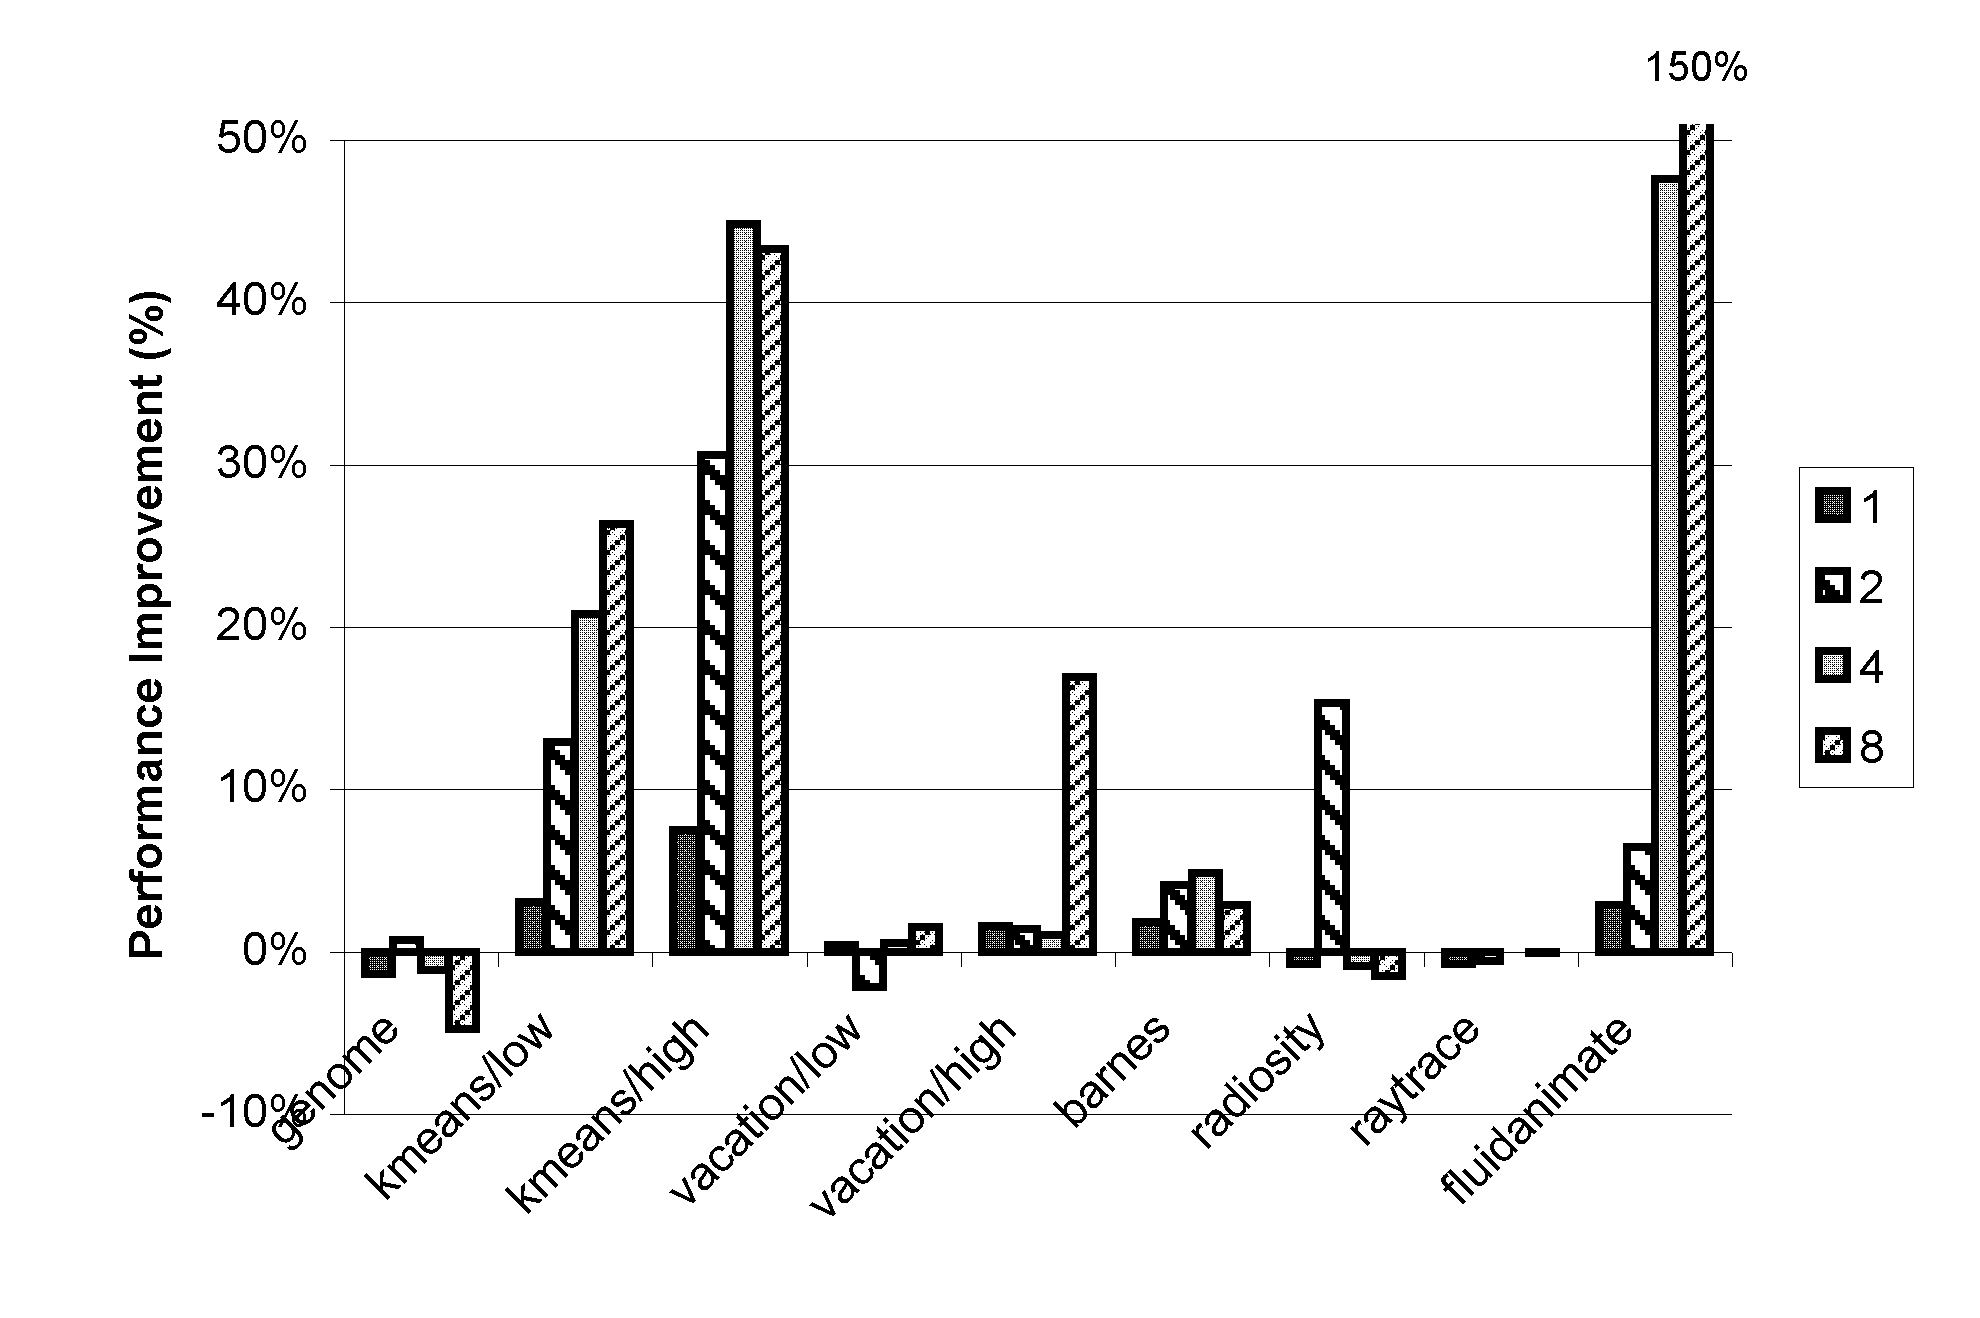
\includegraphics[width=250px]{compiler_optimizations.png}
      \caption{Quelle: \protect\cite[Abbildung 13]{IntegrTMC++}}
      \label{fig:compiler_optimizations}
  \end{figure}
\end{frame}

\end{document}
